%------------------------------------------%
% Cannabis Data Science
% Saturday Morning Statistics
% 11/20/2021
%
% FIXME: Add bibliography
% https://tex.stackexchange.com/questions/148893/package-biblatex-error-incompatible-package-ucs-begindocument?noredirect=1&lq=1
% https://tex.stackexchange.com/questions/261595/how-to-rerun-biber-on-the-file
% https://tex.stackexchange.com/questions/229638/package-biblatex-warning-babel-polyglossia-detected-but-csquotes-missing
% https://tex.stackexchange.com/questions/49610/use-biblatex-and-utf8
% https://stackoverflow.com/questions/1507672/putting-citation-text-on-same-slide-with-latex-beamer
%------------------------------------------%
\documentclass[xcolor={dvipsnames}]{beamer}
\hypersetup{pdfpagemode=FullScreen}
\mode<presentation> %TEMPLATE
{ \usetheme{Boadilla}
  \usecolortheme{orchid}
  \usefonttheme{default}
  \setbeamertemplate{navigation symbols}{}
  \setbeamertemplate{caption}[numbered]} 
\usepackage[english]{babel}
\usepackage[utf8x]{inputenc}
\setbeamersize{text margin left=0.5in,text margin right=0.5in}

\usepackage[dvipsnames]{xcolor}
\definecolor{DarkGreen}{RGB}{2, 48, 32}
\definecolor{CalyxGreen}{RGB}{34, 153, 84}
\definecolor{DarkOrange}{RGB}{199, 0, 57}
\definecolor{LightOrange}{RGB}{255, 87, 51}
\definecolor{LightGreen}{RGB}{218, 247, 166}
\definecolor{LightYellow}{RGB}{255, 195, 0}

\setbeamercolor*{palette primary}{bg=LightGreen, fg = DarkGreen}
\setbeamercolor*{palette secondary}{bg=LightGreen, fg=DarkGreen}
\setbeamercolor*{palette tertiary}{bg=LightGreen, fg = DarkGreen}
%\setbeamercolor*{palette quaternary}{bg=myNewColorD, fg = green}

%------------------------------------------%
% FIXME: Bibliography
%------------------------------------------%
%\usepackage{csquotes}
%\usepackage[style=verbose]{biblatex}
%\addbibressource{presentation-bib.bib}

%------------------------------------------%
% Packages
%------------------------------------------%
\usepackage{amsmath}
\renewcommand*\footnoterule{} %No sperating line on footnote
\usepackage{mathtools} %ANNOTATING EQUATIONS
\usepackage{hhline} %DOUBLBARS
\usepackage[super]{nth}
\usepackage{graphicx, caption, subcaption}

%------------------------------------------%
% Commands
%------------------------------------------%
\newcommand\T{\rule{0pt}{2.5ex}} %TOPSTRUT
\newcommand\B{\rule[-1.25ex]{0pt}{0pt}} %BOTTOMSTRUT
\newenvironment<>{varblock}[2][.9\textwidth] %RESIZED BLOCKS
  {\setlength{\textwidth}{#1}
  \begin{actionenv}#3
    \def\insertblocktitle{#2}\par
    \usebeamertemplate{block begin}}
  {\par\usebeamertemplate{block end}
  \end{actionenv}}
\defbeamertemplate{enumerate item}{largeball} %LARGE BALLS
{\begin{pgfpicture}{-1ex}{-0.65ex}{1.5ex}{1.5ex}
\usebeamercolor[fg]{item projected}
{\pgftransformscale{2.5}\pgftext{\Large\pgfuseshading{bigsphere}}}
{\pgftransformshift{\pgfpoint{0pt}{0.5pt}}
\pgftext{\usebeamerfont*{item projected}\small\insertenumlabel}}
\end{pgfpicture}}
\usepackage{tikz} % FANCY ARROWS
\usepackage{xparse}
\NewDocumentCommand\UpArrow{O{2.0ex} O{black}}{%
   \mathrel{\tikz[baseline] \draw [->, line width=0.5pt, #2] (0,0) -- ++(0,#1);}} % FANCY UPARROW
\NewDocumentCommand\DownArrow{O{2.0ex} O{black}}{%
   \mathrel{\tikz[baseline] \draw [<-, line width=0.5pt, #2] (0,0) -- ++(0,#1);}} % FANCY DOWNARROW
%\vskip 1cm
\makeatletter
\newcommand{\LeftEqNo}{\let\veqno\@@leqno}%LEFT EQUATION #'s
\makeatother

%------------------------------------------%
% Title
%------------------------------------------%
\title[Saturday Morning Statistics]{}
\author{Cannabis Data Science}
\institute[]{\Large Saturday Morning Statistics}
\date{November \nth{20}, 2021}
\begin{document}
\begin{frame}{}
  
\includegraphics[scale=0.075]{images/logos/cannlytics_logo_with_text_light.png}
  \titlepage
\end{frame}

%------------------------------------------%
% Introduction
%------------------------------------------%

% TODO: Discuss Structural Breaks

% TODO: Discuss Difference-in-difference models

\section{Introduction}

% Applications

\begin{frame}{}

{\large Cannabis License Applications in Massachusetts}\vspace{0.5\baselineskip}\\

\begin{figure}
    \begin{subfigure}[t]{1\textwidth}
      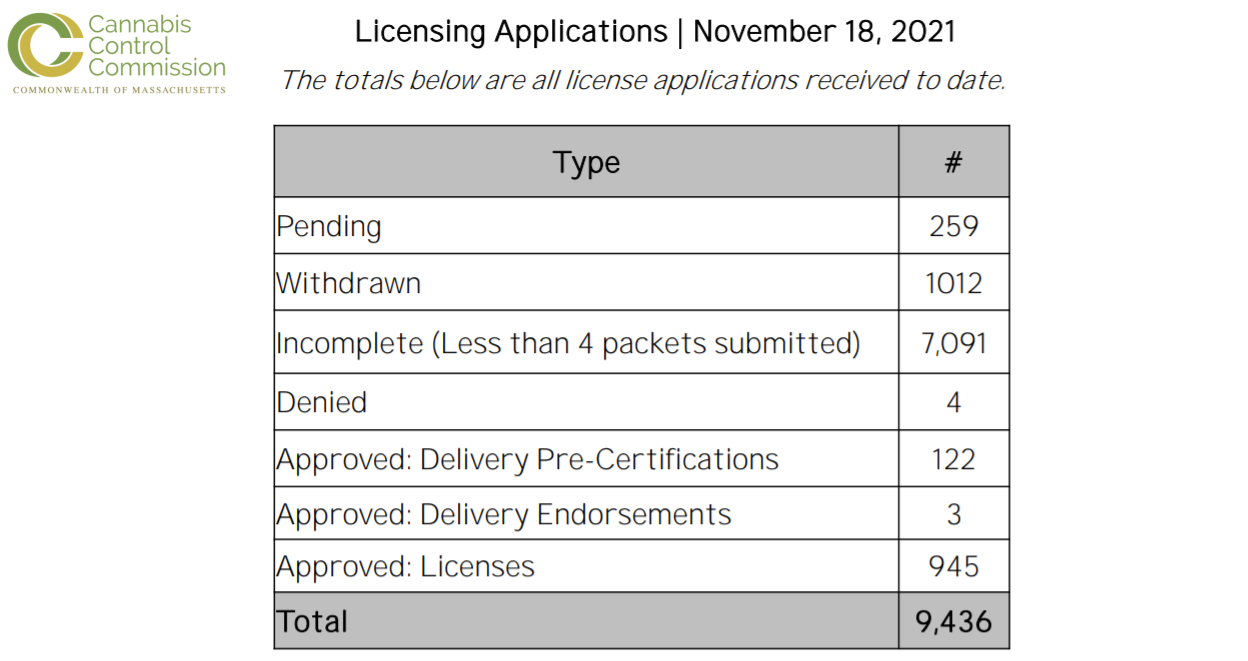
\includegraphics[width=\textwidth]{images/ma_applications.png}
    \end{subfigure}
\end{figure}


\end{frame}

% Stages

\begin{frame}{}

{\large Approved Cannabis Licenses in Massachusetts}\vspace{0.5\baselineskip}\\

\begin{figure}
    \begin{subfigure}[t]{1\textwidth}
      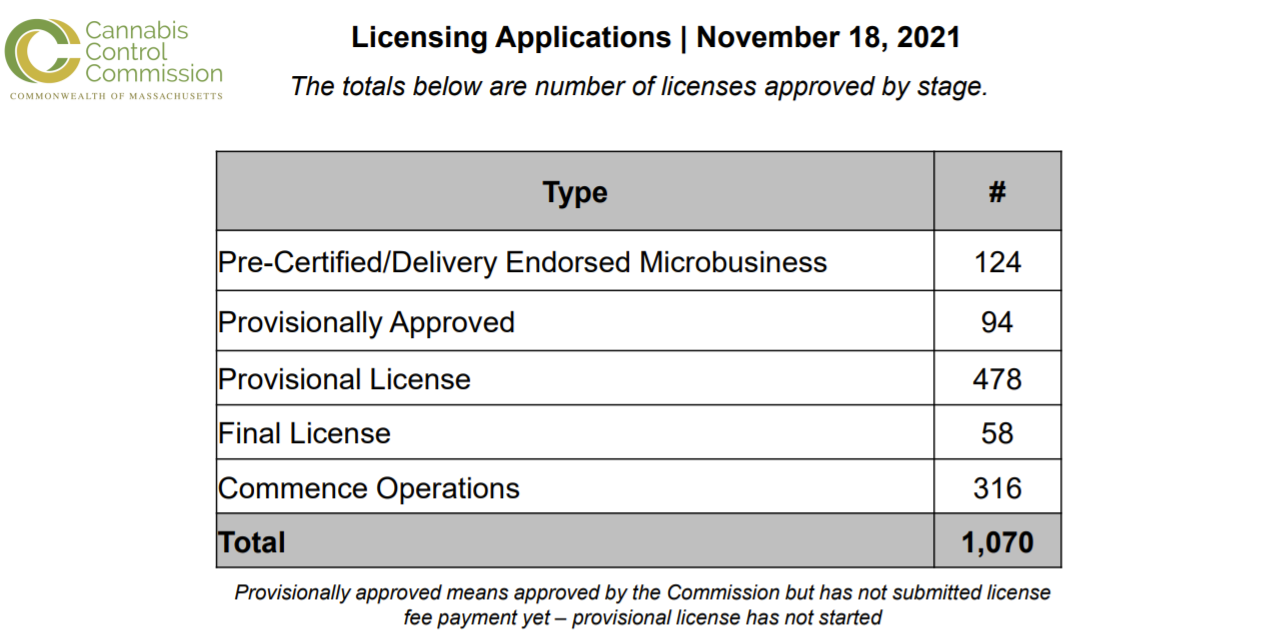
\includegraphics[width=\textwidth]{images/ma_applications_stages.png}
    \end{subfigure}
\end{figure}


\end{frame}

% Types

\begin{frame}{}

{\large Cannabis Licenses by Type in Massachusetts}\vspace{0.5\baselineskip}\\

\begin{figure}
    \begin{subfigure}[t]{1\textwidth}
      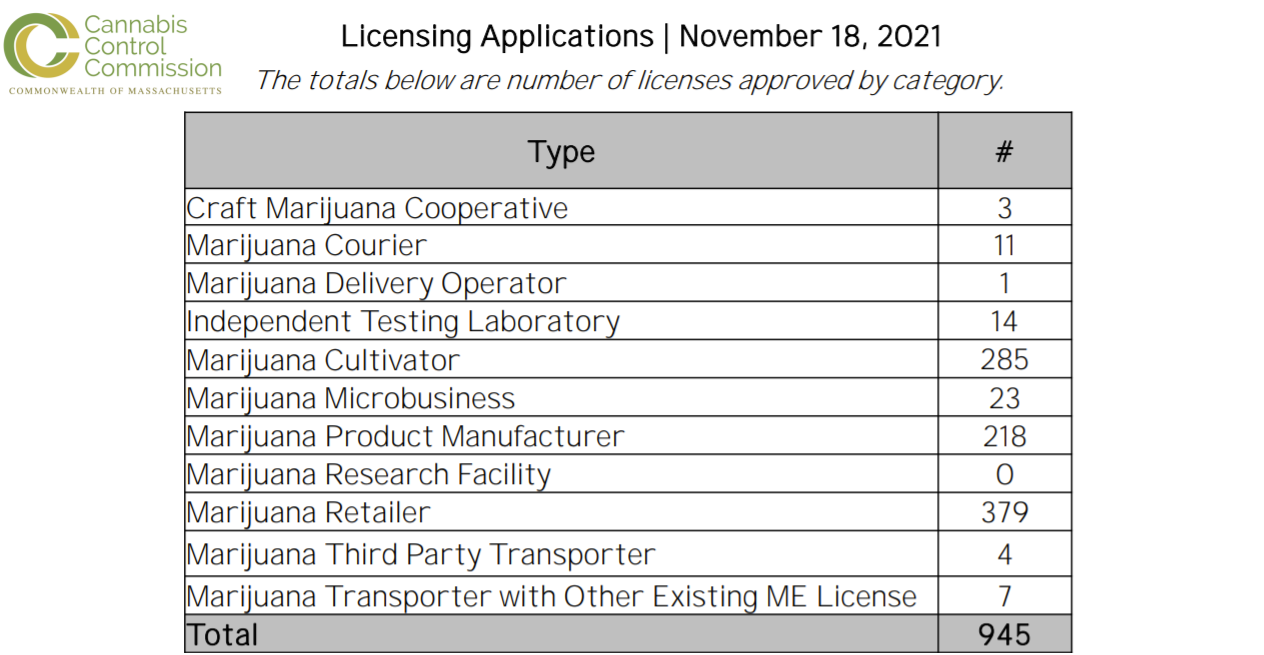
\includegraphics[width=\textwidth]{images/ma_applications_types.png}
    \end{subfigure}
\end{figure}


\end{frame}

% Count

\begin{frame}{}

{\large Cannabis Licenses Approval Stage in Massachusetts}\vspace{0.5\baselineskip}\\

\begin{figure}
    \begin{subfigure}[t]{1\textwidth}
      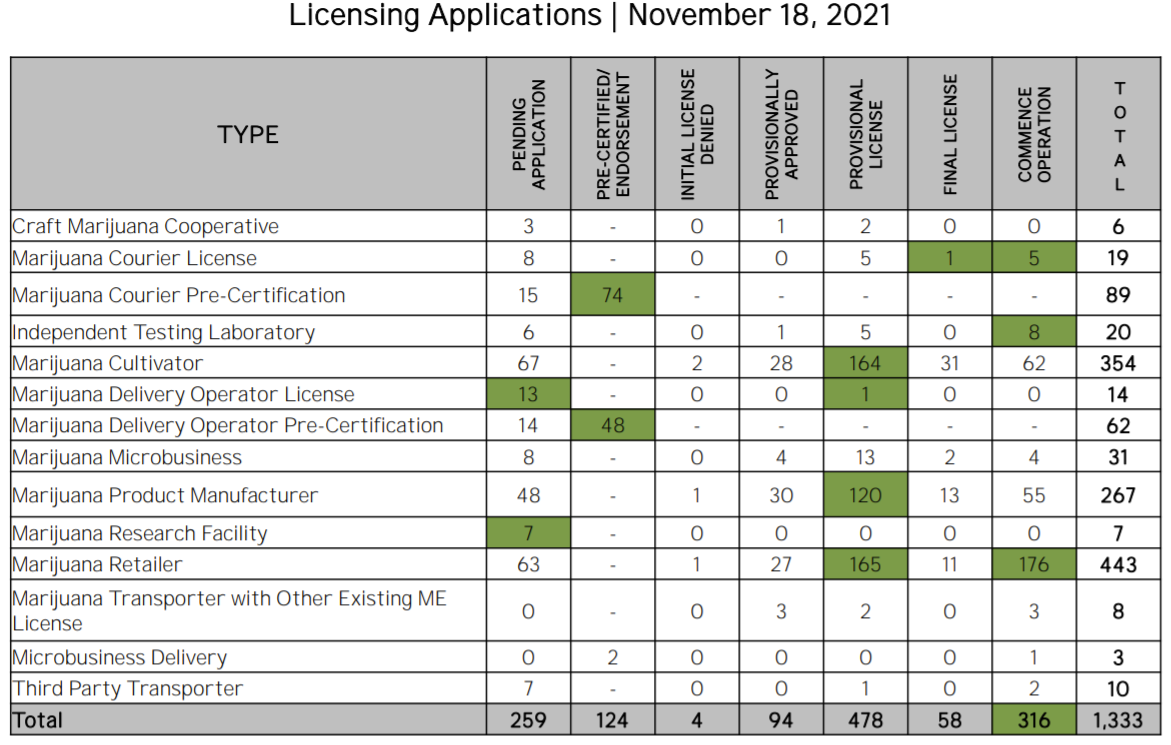
\includegraphics[width=\textwidth]{images/ma_licensees_stage_count.png}
    \end{subfigure}
\end{figure}


\end{frame}


% Cultivation Sq. Fft

\begin{frame}{}

{\large Cultivation in Massachusetts}\vspace{0.5\baselineskip}\\

\begin{figure}
    \begin{subfigure}[t]{1\textwidth}
      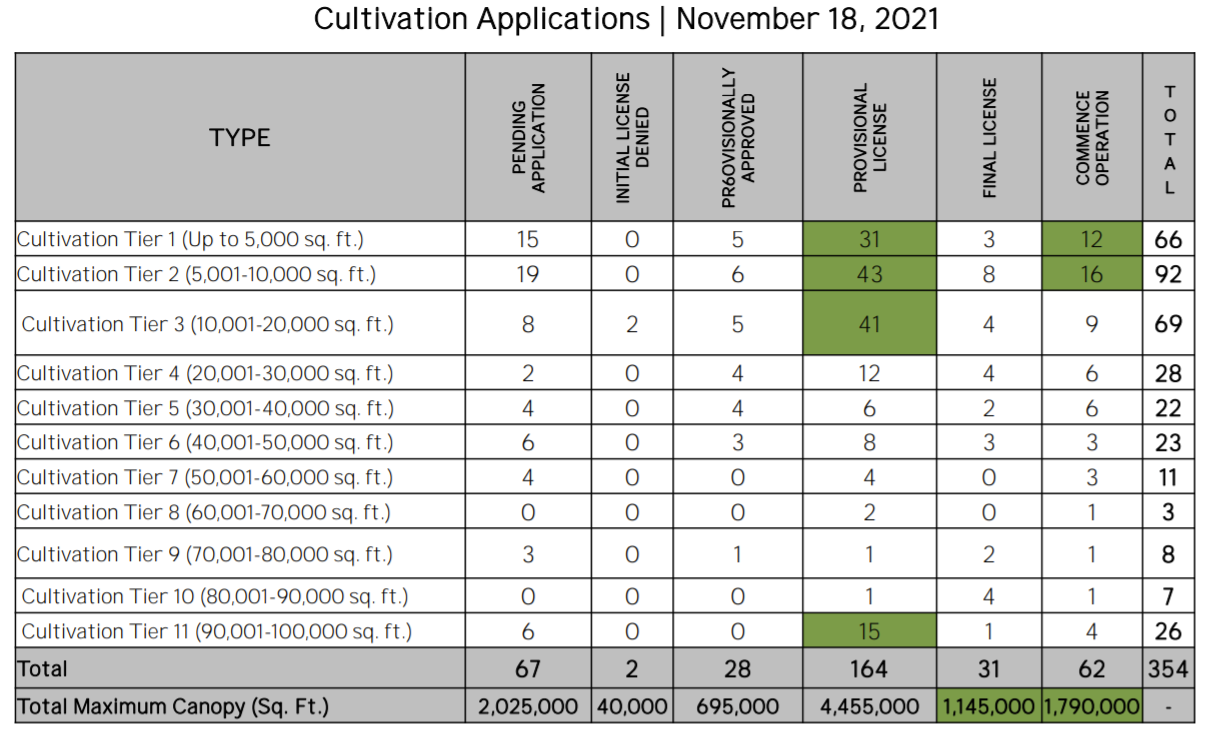
\includegraphics[width=\textwidth]{images/ma_cultivation_sq_ft.png}
    \end{subfigure}
\end{figure}


\end{frame}

% DBEs

\begin{frame}{}

{\large Adult-Use Disadvantaged Business Enterprise (DBE) Statistics}\vspace{0.5\baselineskip}\\


\textit{``The Cannabis Control Commission is dedicated to supporting full and robust industry participation by minorities, women, and veterans. Policies and procedures have been developed to encourage the involvement of people from communities that have previously been disproportionately harmed by marijuana prohibition and enforcement. The licensing process requires all operating marijuana establishments to positively impact those communities. Success will be measured in terms of ownership, employment, and ancillary contributions by these mandated categories of participants in the industry, as well as tangible benefits provided by licensees to disproportionately impacted communities.''}


\end{frame}


% DBE Cities

\begin{frame}{}

{\large DBE Cities}\vspace{0.5\baselineskip}\\

\begin{figure}
  \caption*{Massachusetts Cannabis Control Commission Areas of Disproportionate
Impact}
    \begin{subfigure}[t]{\textwidth}
      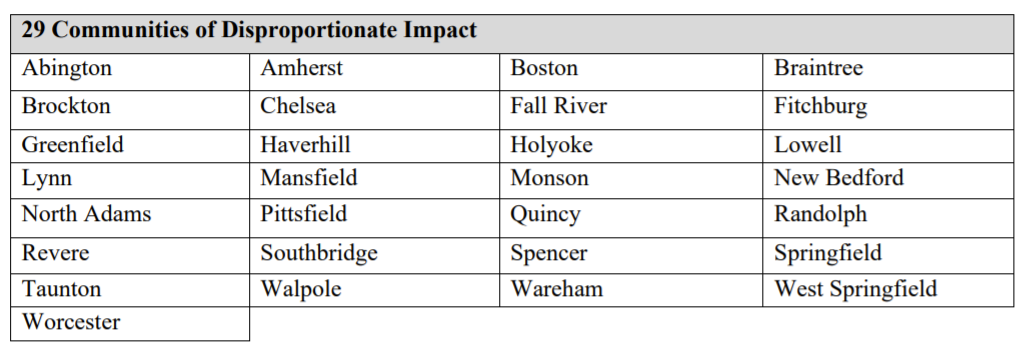
\includegraphics[width=\textwidth]{images/dbe_cities.png}
    \end{subfigure}
\end{figure}

\end{frame}

\section{Statistics}

% Variance

\begin{frame}{}

{\large Variance}\vspace{0.5\baselineskip}\\

\begin{figure}
    \begin{subfigure}[t]{0.6\textwidth}
      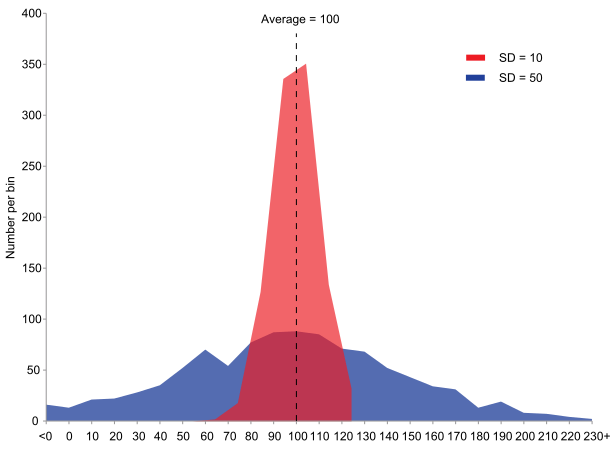
\includegraphics[width=\textwidth]{images/comparison_standard_deviations.png}
    \end{subfigure}
    \caption*{Example of samples from two populations with the same mean but different variances. The red population has mean 100 and variance 100 (SD=10) while the blue population has mean 100 and variance 2500 (SD=50).}
\end{figure}

\end{frame}

% Pearson Correlation Coefficient

\begin{frame}{}
{\large Pearson Correlation Coefficient}\vspace{0.5\baselineskip}

\begin{figure}
    \caption*{Population correlation coefficient}
    \begin{subfigure}[t]{0.4\textwidth}
      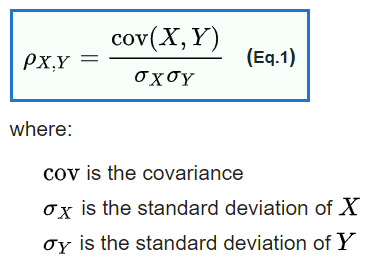
\includegraphics[width=\textwidth]{images/population_correlation_coefficient.png}
    \end{subfigure}
\end{figure}

\begin{figure}
    \caption*{Sample correlation coefficient}
    \begin{subfigure}[t]{0.6\textwidth}
      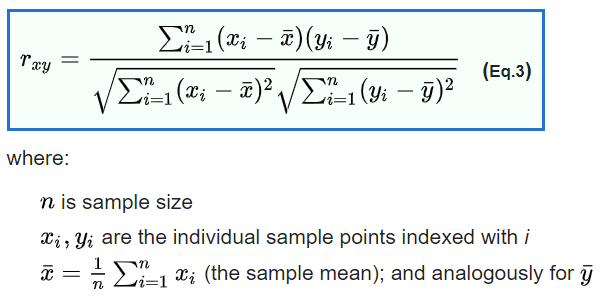
\includegraphics[width=\textwidth]{images/sample_correlation_coefficient.png}
    \end{subfigure}
\end{figure}

\end{frame}

% ANOVA

\begin{frame}{}

\large{Analysis of variance (ANOVA)}\vspace{0.5\baselineskip}

\begin{itemize}

\item A statistical test of whether two or more population means are equal.

\item Generalizes the $t$-test beyond two means,

\end{itemize}

\begin{figure}
    \caption*{Hypothesis Test Type Errors}
    \begin{subfigure}[t]{0.6\textwidth}
      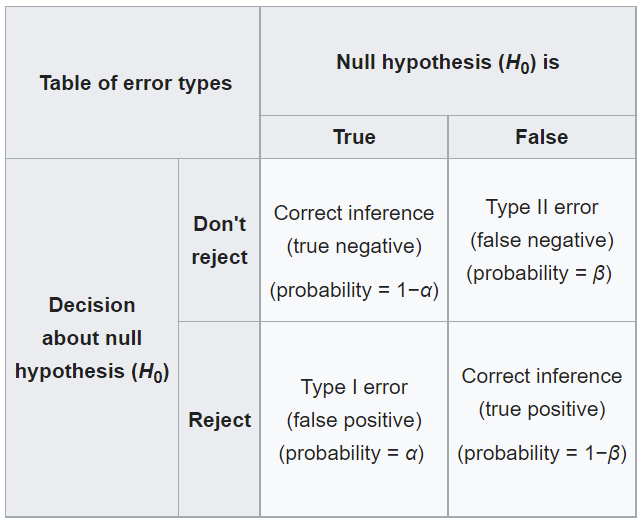
\includegraphics[width=\textwidth]{images/hypothesis_test_error_types.png}
    \end{subfigure}
\end{figure}

\end{frame}



%\begin{frame}{}
%
%{\large }\vspace{0.5\baselineskip}\\
%
%
%\end{frame}





\section{Application}

%------------------------------------------%
% Takeaway
%------------------------------------------%

\begin{frame}{}

{\large Future work: Look at geographic distribution of licensees}\vspace{0.5\baselineskip}\\

\begin{figure}
    \begin{subfigure}[t]{1\textwidth}
      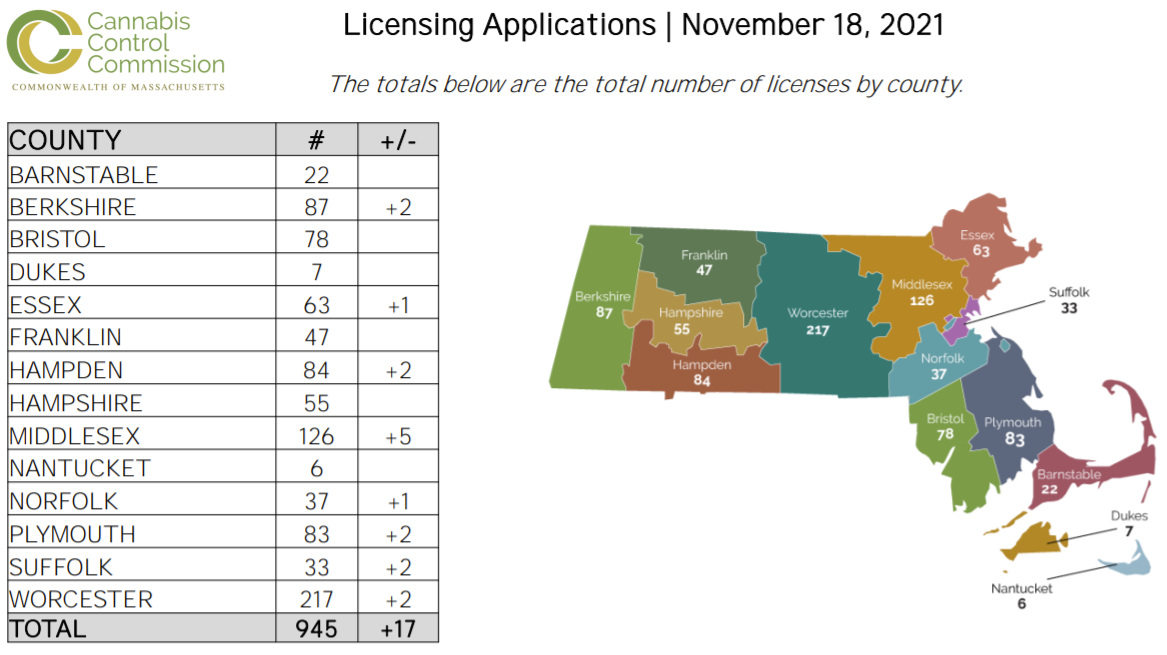
\includegraphics[width=\textwidth]{images/ma_application_map.png}
    \end{subfigure}
\end{figure}

\end{frame}

\begin{frame}{}
\begin{center}
\begin{minipage}{3.85in}
Thank you for coming.
\end{minipage}
\end{center}
\end{frame}

%------------------------------------------%
\end{document}
%------------------------------------------%
